%%%%%%%%%%%%%%%%%%%%%%%%%%%%%%%%%%%%%%%%%%%%%%%%%%%%%%%%%%%%%%%%%%%%%%%%%%%%%%%%
%% 
\cleardoubleoddpage%  Make sure to start each chapter on a new odd page
\chapter{Methodology}

\section{Dataset}
\subsection{Definition}
The Respiratory Sound Database was established for the 2017 International Conference on Biomedical Health Informatics~\cite{rocha2018alpha}. It comprises an open-access collection of audio recordings from 126 patients captured via electronic stethoscopes. These recordings encompass a diverse patient demographic, varying in gender and age, and were obtained using different recording devices containing typical clinical environmental noise.\\
The dataset includes individuals both with and without respiratory diseases. It features explicitly patients diagnosed with one of three conditions: Chronic Obstructive Pulmonary Disease (COPD), Lower Respiratory Tract Infection (LRTI), and Upper Respiratory Tract Infection (URTI). Nine hundred twenty recordings were gathered, amounting to 5.5 hours of audio, with individual recordings ranging from 10 to 90 seconds. Each recording contains multiple breathing cycles, encompassing both inhalation and exhalation, and these cycles may be normal or exhibit signs of anomalies such as wheezes or crackles.\\
In the entire dataset, domain experts annotated 6.898 respiratory cycles. Among these, 3.642 cycles show no anomalies, 1.864 contain crackles, 886 feature wheezes, and 506 simultaneously exhibit both crackles and wheezes.

\subsection{Data Splitting}
\label{method:data-splitting}
We divided the dataset into training, validation, and test sets for a semi-supervised learning approach and to assess model generalization. Following the common practice in the 2017 ICBHI Challenge literature, we adopted an 80/20 split (\autoref{fig:split}) between training and test data, focusing on individual breathing cycles. This split ensures comparability with previous studies.
Initially, the dataset underwent a random split, stratified to maintain equal proportions of normal and anomalous samples, resulting in separate training and test sets. Subsequently, the training set was further divided by performing another stratified random split, with 20\% forming the validation set and the remaining 80\% left in the training set cleared of anomalous data to consist solely of normal breathing cycles. We used \lstinline{train_test_split} from the scikit-learn library~\cite{pedregosa2011scikit} to conduct those splits.\\

\begin{figure}[h!]
    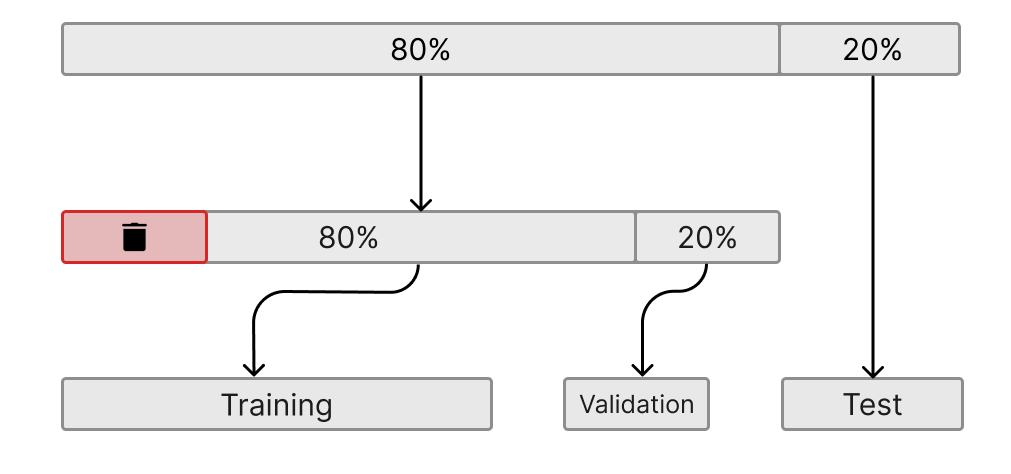
\includegraphics[width=\linewidth]{images/split}
    \caption{
    Visualization of the random 80/20 data split. The red data points get discarded
}\label{fig:split}
\end{figure}

We acknowledge the limitations of this approach. Notably, excluding 2.084 anomalous samples from the training set might affect the model's generalization ability. While reallocating these to the validation or test sets could improve generalization assessment, it raises concerns about data imbalance. Additionally, the initial splitting at the breathing cycle level poses a risk of data leakage, as cycles from the same recording could be distributed across training and test sets, potentially overestimating model performance metrics.\\
To mitigate this, the dataset creators suggested a 60/40 recording-level split where a patient's recording can only appear in either data split. We adopted a similar recording-level split, but we allocated 80\% for training and 20\% for testing to keep enough information available in the unsupervised mode. While ensuring a big enough training dataset even after removing anomalous data, this approach also minimizes data leakage.\\
By employing both splitting strategies, we aim to align our methodology with existing literature and robustly evaluate our model's performance, particularly regarding data leakage prevention.

\section{Preprocessing}
\label{method:preprocessing}
Effective preprocessing is crucial for transforming raw audio data into a format suitable for our machine-learning models. This section outlines the steps taken to achieve this.
Initially, we loaded audio files, each comprising multiple respiratory cycles, along with their corresponding annotation files. These annotations, indicating each cycle's start and end times and the presence of crackles or wheezes, enabled us to extract individual cycles and assign binary labels (1 for abnormal cycles with crackles or wheezes and 0 for normal cycles).\\
Given the dataset's variety in sampling rates across different electronic stethoscopes, a uniform sampling rate was necessary. According to similar work~\cite{cozzatti2022variational,serbes2018automated} and considering the Nyquist Theorem~\cite{por2019nyquist}, we standardized all audio samples to a 4000 Hz sampling rate. This rate effectively captures wheezing sounds (with significant components below 2000 Hz), ensuring that both wheezes and crackles are accurately represented without aliasing.\\
To accommodate the fixed-size input requirement of our models, we normalized the length of respiratory cycles, which ranged from 0.2 seconds to 16.2 seconds, to a consistent 5s. The normalization was achieved by truncating longer sequences and zero-padding shorter ones.\\
Subsequently, we computed 13 MFCCs for each audio sample using PyTorch's~\cite{paszke2019pytorch} \lstinline{torchaudio.transforms.MFCC} implementation. Adjustments to the underlying spectrogram calculations included setting the number of mels to 64, the size of the fast Fourier transform to 256 with a hop length of 128 and a maximum frequency of 2000 Hz. These parameters align with the implementation of Gairola et al. (2021).\\
We then applied the \lstinline{torchaudio.transforms.AmplitudeToDB} transformation to scale the amplitude valued logarithmically. The final preprocessing step involved standardizing the MFCCs to have zero mean and unit standard deviation, preparing them for efficient model processing.

% Maybe I need to mention the [:128]

\section{Detailed Overview of the Models}
In our research, we explored two distinct models to evaluate the efficacy of reconstruction-based and density estimation-based approaches in detecting anomalies in respiratory sounds. Our goal was to maintain consistency in training procedures and preprocessing across both models to ensure fair comparability. However, it is important to note that the architectures of these models are inherently different, and we will delve into the specifics of each.

\subsection{Implementation of the VAE}
The Variational Autoencoder (VAE) serves as our reconstruction-based model. It inputs Mel Frequency Cepstral Coefficients (MFCCs) and outputs reconstructed MFCCs of the same dimension. We began with the well-established DCGAN architecture and adapted it for one-dimensional convolution along the time axis.\\\\
\textbf{Encoder}: The Encoder is composed of five consecutive convolutional layers. Each layer includes a one-dimensional convolution (kernel size 4, stride 2, padding 1), followed by batch normalization and a LeakyReLU activation function with $p=0.2$. After the convolution, there are two linear layers: one outputs the mean ($\mu$), and the other outputs the log-variance ($log(var)$). This setup is designed to model a Gaussian distribution in the latent dimension $z$, with $log(var)$ enhancing numerical stability.\\\\
\textbf{Sampling and Reparametrization Trick}: We encounter a challenge in sampling from this Gaussian distribution, as it is not a differentiable process, which is essential for gradient-based optimization. To address this, we use the reparametrization trick. This method introduces a deterministic noise variable ($\epsilon$) and computes the latent sample as $z=\mu + \sigma \cdot \epsilon$, enabling differentiability and backpropagation.\\\\
\textbf{Decoder}: The Decoder mirrors the Encoder, comprising five convolutional layers. The activation function is replaced with standard ReLU and the last convolutional layer, as it is the output layer of the Decoder, does not use batch normalization and has linear output activation. A linear layer initially processes the latent space sample, reshaping it for compatibility with the convolutional layers.\\\\
\textbf{Initialization and Loss Function}: We initialize all layer weights using the Xavier method. We combine mean squared error (MSE) loss for the reconstruction error and the Kullback-Leibler divergence (KLD) for a measurement of how well the output distribution of the Encoder aligns with the standard Gaussian distribution. The final loss is the weighted sum of both losses $Loss=\alpha \cdot MSE + (\alpha - 1) \cdot KLD$, with $\alpha$ as the weight.

\subsection{Implementation of the GMADE}
The Group Masked Autoencoder for Density Estimation (GMADE) represents our alternative model for respiratory sound anomaly detection, operating on the principles of autoregressive density estimation.\\\\
\textbf{Model Architecture}: At its core, GMADE uses a modified linear autoencoder structure, where we replace the traditional linear layers with MaskedLinear layers (\autoref{code:maskedlinear}) that add the functionality for a configurable weight mask to enforce the autoregressive property. The model is constructed as a feed-forward network with several MaskedLinear layers followed by ReLU activation functions. The final output layer omits the ReLU activation for linear output.
\begin{lstlisting}[label=code:maskedlinear,language=Python,caption={MaskedLinear PyTorch implementation as described by Karpathy, Andrej (2018)~\cite{githubMADE}}]
    class MaskedLinear(nn.Linear):    
        def __init__(self, in_features, out_features, bias=True):
            super().__init__(in_features, out_features, bias)        
            self.register_buffer('mask', torch.ones(out_features, in_features))
        
        def set_mask(self, mask):
            self.mask.data.copy_(torch.from_numpy(mask.astype(np.uint8).T))
            
        def forward(self, input):
            return F.linear(input, self.mask * self.weight, self.bias)
\end{lstlisting}

\textbf{Mask Generation and Update}: A significant aspect of the implementation is the generation and updating of the weight masks as they determine the connections between neurons in subsequent layers. The masks are dynamically generated based on the input ordering and connectivity of neurons and allow for varying ordering strategies, such as causal, backward, and middle frame orderings. The model can generate multiple masks to allow for the ensemble of different neuron connectivities. To illustrate the implementation in \autoref{code:updatemask}, we consider the case of using one mask.
\begin{lstlisting}[label=code:updatemask, language=Python,caption={PyTorch implementation of the mask generation, adapted from Karpathy, Andrej (2018)~\cite{githubMADE}}]
    def update_masks(self):
        # define the number of linear layers of the model
        L = len(self.hidden_sizes)
        
        # create a numpy random number generator instance
        rng = np.random.RandomState(self.seed)

        # define input order
        # here: forward ordering for 5 frames and 13 MFCCs
        expanded_order = np.tile([0, 1, 2, 3, 4], 13)
        
        # sample the order of the inputs and the connectivity of all neurons
        # store each layer's weights in self.m
        self.m[-1] = expanded_order # input ordering for first layer
        for l in range(L):
            # for each layer, assign label ranging from smallest label
            # of previous layer to the number of groups - 1 at random
            self.m[l] = rng.randint(self.m[l-1].min(), self.num_frames-1, size=self.hidden_sizes[l])
        
        # construct the mask matrices according to the MADE definition
        masks = [self.m[l-1][:,None] <= self.m[l][None,:] for l in range(L)]
        # strictly larger in the case of output layer
        masks.append(self.m[L-1][:,None] < self.m[-1][None,:])
        
        # set the masks in all MaskedLinear layers
        layers = [l for l in self.net.modules() if isinstance(l, MaskedLinear)]
        for l,m in zip(layers, masks):
            l.set_mask(m)
\end{lstlisting}
\textbf{Loss Function}: We used the Gaussian Negative Log Likelihood (GaussianNLL) for training GMADE. This choice aligns with the model's focus on density estimation, as it effectively measures how well the model predicts the probability distribution of the output given the input.
%% 
%%%%%%%%%%%%%%%%%%%%%%%%%%%%%%%%%%%%%%%%%%%%%%%%%%%%%%%%%%%%%%%%%%%%%%%%%%%%%%%%
